\documentclass[12pt, a4paper]{article}
\usepackage{graphicx}
\usepackage[hidelinks]{hyperref}
\usepackage{indentfirst}
\usepackage[indonesian]{babel}

\makeatletter
\renewcommand{\maketitle}{\bgroup\setlength{\parindent}{0pt}
\begin{flushleft}
  \LARGE\textbf{\@title}

  \normalsize\@author
\end{flushleft}\egroup
}

\title{Resume Telemedicine}
\author{Aufa Nabil Amiri - 0721 17 4000 0029}
\date{}

\begin{document}
\maketitle

\section*{Aspek Dalam Telemedicine}

Aspek yang dipakai adalah dalam penggunaan \textit{cloud computing} untuk memproses dan menyimpan data dari 12 titik EKG. Fokus dari penelitian yang ditulis berfokus pada \textit{tele-consultation} pada pasien selama di ambulan, antara dokter yang sedang ditempat dengan dokter senior yang sedang tidak ditempat, juga digunakan antar rumah sakit.

\section*{Bagaimana Melakukan}

\begin{figure}[h!]
    \begin{center}
        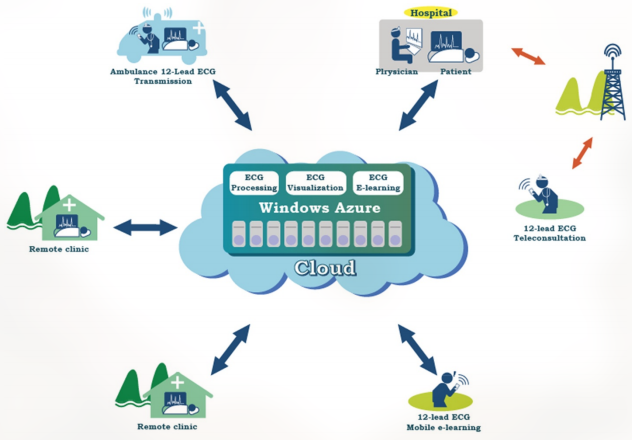
\includegraphics[width=\linewidth]{grafik2.png}
    \end{center}
\end{figure}

Sebuah mesin ECG yang sudah terkoneksi dengan internet, baik itu melalui kabel seperti RS232 maupun melalui jaringan nirkabel akan melakukan konversi data ke XML-ECG, SCP-ECG atau DICOM-ECG. Data tersebut akan dikirim melalui TCP/IP.

Sumber data yang berupa teks yaitu XML-ECG maupun yang berupa \textit{blob} yaitu SCP-ECG dan DICOM-ECG akan diproses dan disimpan dalam bentuk gelombang dengan memanfaatkan \textit{cloud computing} berupa Windows Azure. Keuntungan dari menggunakan Windows Azure adalah tidak adanya \textit{vendor lock-in} karena basis dari Windows Azure sendiri adalah MS-SQL. Sehingga, apabila suatu rumah sakit ingin menggunakan sistem mereka sendiri, bisa menggunakan MS-SQL sebagai basis datanya.

Seorang dokter yang sedang tidak berada di rumah sakit dapat menggunakan jaringan \textit{mobile data} sebagai pengganti jaringan rumah sakit. Untuk mengakses sistem \textit{telemedicine} ini, dokter hanya perlu melakukan login melalui perangkat masing - masing dan data akan sudah didapat.

Data yang sudah disimpan ke dalam server, dapat digunakan dengan berbagai keperluan, seperti \textit{ECG Processing} yaitu membahas suatu kasus pasien untuk memberikan suatu treatment secara \textit{online}. Juga terdapat \textit{ECG Visualization} untuk menampilkan grafik gelombang EKG yang sudah diperoleh. Dan terakhir \textit{ECG E-Learning}, dimana grafik - grafik EKG yang disimpan, dapat digunakan sebagai media pembelajaran.

\section*{Teknologi yang Digunakan}

\begin{enumerate}
    \item \textbf{Windows Azure}

          Windows Azure merupakan platform \textit{cloud computing} yang dibuat oleh Microsoft dan memiliki pengguna yang cukup banyak. Digunakan sebagai tempat penyimpanan basis data yang digunakan.

    \item \textbf{MS-SQL}

          Merupakan perangkat lunak basis data yang digunakan dalam implementasi \textit{telemedicine} ini. Untuk kemudahan akses, MS-SQL di\textit{host} dengan menggunakan Windows Azure. Namun apabila pihak rumah sakit ingin menggunakan jaringan internal, dapat dilakukan dengan memasang MS-SQL ke dalam jaringan tersebut.

    \item \textbf{12-lead ECG}

          Digunakan sebagai sumber data yang akan disimpan dalam MS-SQL. Terdapat beberapa standar yang digunakan seperti XML-ECG oleh Philips, SCP-ECG oleh HP, dan DICOM-ECG oleh Mortara. Ketiganya merupakan standar yang sering ditemui di rumah sakit umum.

\end{enumerate}

\section*{Bagaimana Pemanfaatannya}
Pemanfaatannya sendiri sangat banyak, dengan menggunakan \textit{telemedicine} seperti ini, suatu rumah sakit dapat bekerja sama satu sama lain dan meningkatkan tingkat kesembuhan dimanapun lokasi rumah sakit tersebut.

\section*{Referensi}

\noindent Hsieh, Jc., Hsu, MW. A cloud computing based 12-lead ECG telemedicine service. BMC Med Inform Decis Mak 12, 77 (2012). \url{https://doi.org/10.1186/1472-6947-12-77}

\end{document}